\begin{frame}{Overview}

\begin{itemize}
\vfill
    \item From previously:
\begin{enumerate}
    \item Equations
    \item Substitution
    \item $\bot_i$
    \item Modes
    \item Algorithms
\end{enumerate}

\vfill
\item Algorithms:
\begin{enumerate}
    \item Construct $C$ from $\bot_i$
    \item Cover set algorithm
\end{enumerate}

\vfill
\item Difficulties:
\begin{enumerate}
    \item $\bot_i$
    \item Progol
\end{enumerate}
\vfill
\end{itemize}

\end{frame}


\begin{frame}{Previously: equations}

\begin{align}
B \land H \quad &\models \quad E \label{eq1} \\
B \land \overline{E} \quad &\models \quad \overline{H} \label{eq2} \\
B \land \overline{E} \quad &\models \quad \overline{\bot} \label{eq3} \\
\overline{\bot} \quad &\models \quad \overline{H} \label{eq4} \\
H \quad &\models \quad \bot \label{eq5} \\
B \land \overline{e} \land \bot \quad &\vdash_h \quad \square
\end{align}

\begin{itemize}
\item $B$: background knowledge
\item $H$: hypothesis
\item $E$: examples
\item $\overline{\bot}$: set of all true literals (wrt. $B \land \overline{E}$)
\item $\bot$: most specific clause
\end{itemize}

\end{frame}

\begin{frame}{Previously: substitution}
    
\begin{block}{Substitution}
Let $\theta$ be a substitution of the form \{$v_1/t_1, ..., v_n/t_n$\}. \\
Let $F$ be an arbitrary atom. \\
$F\theta$ is the atom $F$ where each of its variable $v_i$ have been replaced by $t_i$.
Ex: 
\begin{itemize}
    \item $F: parent(X,Y)$
    \item $\theta: \{X/\text{jean},\ Y/\text{bob}\}$
    \item $F\theta: parent(\text{jean},\text{bob})$
\end{itemize}
\end{block}

\begin{block}{Clause substitution}
The same can be done for a clause $C$:
\begin{itemize}
    \item $F: parent(X,Y) :- father(X,Y).$
    \item $\theta: \{X/\text{jean},\ Y/\text{bob}\}$
    \item $F\theta: parent(\text{jean},\text{bob}) :- father(\text{jean},\text{bob}).$
\end{itemize}
\end{block}
    
\end{frame}

\begin{frame}{Previously: $\bot_i$}

\begin{block}{Depth $d(v)$}
\[
    d(v) = 
\begin{cases}
    0, & \text{if } v \text{ is in the head of }C\\
    (\min_{u\in U_v} d(u)) +1,              & \text{otherwise}
\end{cases}
\] where $U_v$ are the variables in atoms in the body of $C$ containing $v$.\\
Ex:
\begin{itemize}
    \item C: p(A) :- p(A,B), g(B,C), f(C,D)
    \item $d(A)=1, \ d(B)=2, \ d(C)=3, \ d(D)=3$
\end{itemize}
\end{block}

\begin{itemize}
    \item $\bot$ can have an infinite cardinality
    \item $\bot_i$ is more restrained
    \begin{itemize}
        \item the distance of its variables is $\leq i$
    \end{itemize}
\end{itemize}
    
\end{frame}

\begin{frame}{Previously: modes}

\begin{block}{Horn clause}
$C: A \leftarrow B_1, ..., B_n$
\begin{itemize}
    \item $A$ is the head of clause $C$
    \item $B_1, ..., B_n$ is the body of clause $C$
\end{itemize}
\end{block}
\begin{block}{Mode declaration}
\begin{itemize}
    \item modeh($n$,atom) $|$ modeb($n$,atom)
    \item modeh(*,f(+int,-int)), modeb(*,d(+int,-int))
    \item Use \textit{modeh} for the head of a clause, \textit{modeb} for its body
\end{itemize}
\end{block}    

\end{frame}

\begin{frame}{Previously: modes (ii)}
\begin{block}{Instantiation}
\begin{itemize}
    \item Let $M$ be a set of modes
    \item $m \in M$ is a mode declaration
    \item $a(m)$ is the atom of $m$ with place markers replaced
\end{itemize}
Ex
\begin{align*}
m &= \text{modeh}(*,f(+\text{int},-\text{int})) \\
a(m) &= f(A,B)
\end{align*}
\end{block}
\end{frame}

\begin{frame}{Previously: algorithms}
\begin{itemize}
    \item Three algorithms:
    \begin{itemize}
    \item Cover set algorithm
    \item Construct $\bot_i$
    \item Construct $C$ form $\bot_i$
    \end{itemize}
\end{itemize}    
\end{frame}


\begin{frame}{Algorithms: Cover set algorithm}
    
\begin{algorithm}[H]
\scriptsize
\caption{Cover set algorithm}
\SetKwInOut{Input}{input}
\Input{$h,i,B,M,E$}
\ForAll{$e \in E$}{
Construct $\bot_i$ for $e$ using Algorithms \ref{alg:bot1} and \ref{alg:bot2} \\
Construct state $s$ from $\bot_i$ using Algorithm \ref{alg:C} \\
Let $C'$ be the unflattening of $C(s)$ \\
$B \gets B \cup C'$ \\
$E \gets E - \{e: e\in E, \ B \land \overline{e} \vdash_h \emptyset\}$ \\
}
\end{algorithm}

\end{frame}

\begin{frame}{Algorithms: Construct $C$}

\begin{algorithm}[H]\label{alg:C}
\scriptsize
\caption{Construct $C$}
\SetKwInOut{Input}{input}
\Input{$h, B, e, \bot_i$}
Open $\gets \{\langle\square, \emptyset, 1\rangle\}$, Closed $\gets \emptyset$ \\
\While{True}{
$s \gets $ best(Open) \\
Open $\gets$ Open $- \{s\}$, Closed $\gets$ Closed $\cup \{s\}$ \\
\If{$\neg$ prune($s$)}{
Open $\gets$ $(\text{Open} \cup \rho(s)) - \text{Closed}$ \\
}
\If{terminated(Closed,Open)}{\Return best(Closed)}
\If{Open $=\emptyset$}{
print 'no compression'\\
\Return $\langle e,\emptyset,1 \rangle$\\
}
}

\end{algorithm}

\begin{itemize}
    \item $\rho$ is the refinement operator
\end{itemize}    
\end{frame}


\begin{frame}{Algorithms: Constructing $\bot_i$ (i)}

\begin{algorithm}[H]
\scriptsize
\caption{Construct $\bot_i$ - Part 1}\label{alg:bot1}

Get $m \in M$, modeh such that $a(m) \preceq a$ with substitution $\theta_h$ \\
\If{$\nexists m$}{
\Return $\square$ \\
}
$a_h \gets a(m)$ \\
\For{$v/t \in \theta_h$}{
\If{$v$ corresponds to \#type in $m$}{
Replace $v$ by $t$ in $a_h$ \\
}\Else{
Replace $v$ by $v_k$ in $a_h$, with $k=\text{hash}(t)$ \\
}
\If{$v$ corresponds to +type in $m$}{
Add $v$ to InTerms \\
}
}
Add $a_h$ to $\bot_i$ \\

\end{algorithm}    
    
\end{frame}

\begin{frame}{Algorithms: Constructing $\bot_i$ (ii)}

\scalebox{0.9}{
\begin{algorithm}[H]
\scriptsize
\caption{Construct $\bot_i$ - Part 2}\label{alg:bot2}
\For{$k \gets 1,\dots,i$}{
\ForAll{modeb $m \in M$}{
Let $\{v_1, ..., v_n\}$ be the variables corresponding to +type in $a(m)$ \\
Let $T_i$ be the set of all terms of the type associated with $v_i$ in $m$ \\
$T(m) \gets T_1 \times ... \times T_n$ \\

\ForAll{$\langle t_1,\dots,t_n \rangle \in T(m)$}{
$a_b \gets a(m)$ \\
$\theta \gets \{v_1/t_1,...,v_n/t_n\}$ \\

\If{Prolog succeeds on goal $a_b\theta$}{

Let $\Theta_b$ be the set of answer substitutions \\

\ForAll{$\theta_b \in \Theta_b$}{
\ForAll{$v/t \in \theta_b$}{
\If{$v$ corresponds to \#type in $m$}{
Replace $v$ by $t$ in $a_b$ \\
}\Else{
Replace $v$ by $v_k$ in $a_b$, with $k=\text{hash}(t)$ \\
}
\If{$v$ corresponds to -type}{
Add $v$ to InTerms \\
}
}
}
Add $\overline{a_b}$ to $\bot_i$ \\

}
}
}
}
\Return $\bot_i$

\end{algorithm}
}    
\end{frame}


\begin{frame}{Important numbers}
\begin{figure}
    \centering
    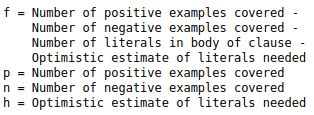
\includegraphics[width=0.5\textwidth]{images/Numbers_progol.png}
    \label{fig:my_label}
\end{figure}    
\end{frame}

\begin{frame}{Example of execution}

\begin{figure}
    \centering
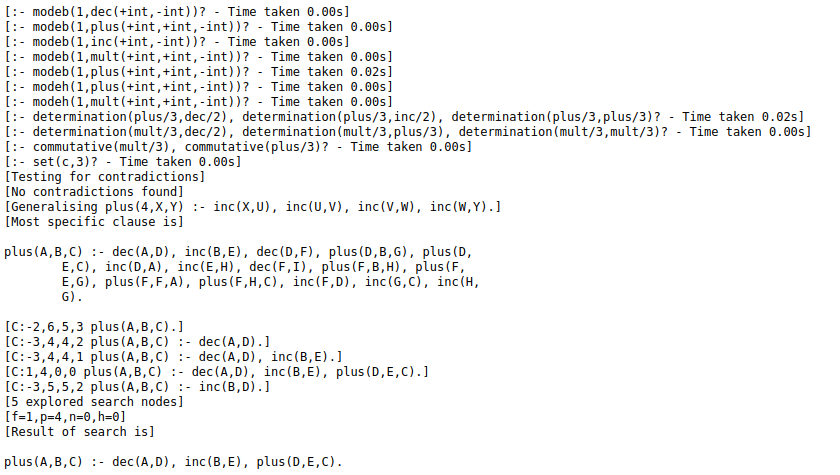
\includegraphics[width=\textwidth]{images/Details_progol.png}
\end{figure}
\end{frame}


\begin{frame}{Difficulties}
    
\end{frame}
